\section{About Us}
\AtBeginSection[]
{
	\begin{frame}<beamer>
		\frametitle{Plan}
		\tableofcontents[currentsection]
	\end{frame}
}

\begin{frame}{About Us}
	\begin{block}{Lutra Consulting}
		\begin{itemize}
			\item Core QGIS developers
			\item General (GIS) software/web development
			\item Support
			\item Training
		\end{itemize}
	\end{block}
\end{frame}

\subsection{QGIS core development}
\begin{frame}{QGIS features we developed}
\begin{block}{Development of:}
	\begin{itemize}
		\item Multi-threaded rendering (2.4)
		\item Legend re-factoring and support for virtual multi-canvas, multi-styling (2.6 - 2.10)
		\item Rule-based labelling (2.12)
		\item Trace digitizing and snap caching (2.14)
		\item For the upcoming 2.16 release:
		\begin{itemize}
			\item Legend item widget tool
			\item Enhancement to the "reshape" digitizing tool
			\item Advanced "preset" settings for the Print Composer
		\end{itemize}		
	\end{itemize}
\end{block}
\end{frame}


\subsection{Public QGIS tools and plugins}
\begin{frame}{Various plugins}
\centering{
\includegraphics[width=0.9\textwidth]{plugins.png}}
\end{frame}

\section{Migration to Open Source GIS}
\subsection{Current state}
\begin{frame}{Current SDI}
	\begin{block}{SDI environments:}
		\begin{itemize}
			\item Proprietary software
			\item Black boxes with Open source components
			\item Hybrid
		\end{itemize}
	\end{block}
\end{frame}

\subsection{Proprietary software}
\begin{frame}{Proprietary software}
	\begin{block}{Pros and Cons}
		\begin{itemize}
			\item Advantages:
			\begin{itemize}
				\item Unified platform
				\item Support and documentation
				\item Usability
			\end{itemize}
			\item Disadvantages
			\begin{itemize}
				\item Dependency
				\item Overall cost
				\item Flexibility
			\end{itemize}
		\end{itemize}
	\end{block}
\end{frame}

\subsection{Black box OS software}
\begin{frame}{Black box OS software}
	\begin{block}{Pros and Cons}
		\begin{itemize}
			\item Advantages:
			\begin{itemize}
				\item Things work
				\item Easy to migrate away
			\end{itemize}
			\item Disadvantages
			\begin{itemize}
				\item Similar cost to Proprietary Software
				\item Not configurable/Customisable
			\end{itemize}
		\end{itemize}
	\end{block}
\end{frame}

\section{Case study - Newcastle City Council}
\subsection{Business Case \& Rational}
\begin{frame}{Business Case \& Rational}
	\begin{block}{Why migrate away:}
		\begin{itemize}
			\item Performance issues
			\item Expensive software
			\item More number of users
			\item Unwanted extras
		\end{itemize}
	\end{block}
\end{frame}

\subsection{Evaluation and pilot study}
\begin{frame}{Evaluation and pilot study}
	\begin{block}{}
		\begin{itemize}
			\item Migrating some data to PostGIS
			\item Migrating power users to QGIS
			\item Identifying blockers
			\item Assessing data \& service compatibility and interoperability
		\end{itemize}
	\end{block}
\end{frame}

\subsection{Full implementation}
\subsubsection{QGIS}
\begin{frame}{Desktopn GIS}
	\begin{block}{Customised QGIS - based on the LTR}
		\begin{itemize}
			\item Resolving issues with the Active Directory
			\item Development of a QGIS plugin for gazetteer
			\item Integration with their OGC services
			\item Fixing bug (backport to QGIS project)
		\end{itemize}
	\end{block}
	\centering{
\includegraphics[width=0.7\textwidth]{b77ada24-3f76-11e5-808f-6686696e19f0.jpg}}
\end{frame}

\begin{frame}{Training}
	\begin{block}{Bespoke training for over 75 users}
		\begin{itemize}
			\item Conversion from previous platform to QGIS
			\item Several new users
		\end{itemize}
	\end{block}
\end{frame}

\subsection{PostGIS}

\subsubsection{Migrating data}

\begin{frame}{PostGIS}
	\begin{block}{Migrating data}
		\begin{itemize}
			\item OS Translator II
			\item ogr2ogr scripts
		\end{itemize}
	\end{block}	
\end{frame}

\begin{frame}{PostGIS}
	\begin{block}{Migrating data}
		\begin{itemize}
			\item Test server
			\item Main server
			\begin{itemize}
				\item with back-up / restore script
			\end{itemize}
		\end{itemize}
	\end{block}	
\end{frame}

\subsubsection{Sync tool with ArcSDE}

\begin{frame}{PostGIS}
	\begin{block}{Sync tool with ArcSDE}
		\begin{itemize}
			\item Waiting for ESRI support (1 year!)
		\end{itemize}
	\end{block}	
\end{frame}

\section{WebGIS and Geoserver}
\begin{frame}{Geoserver}
	\centering{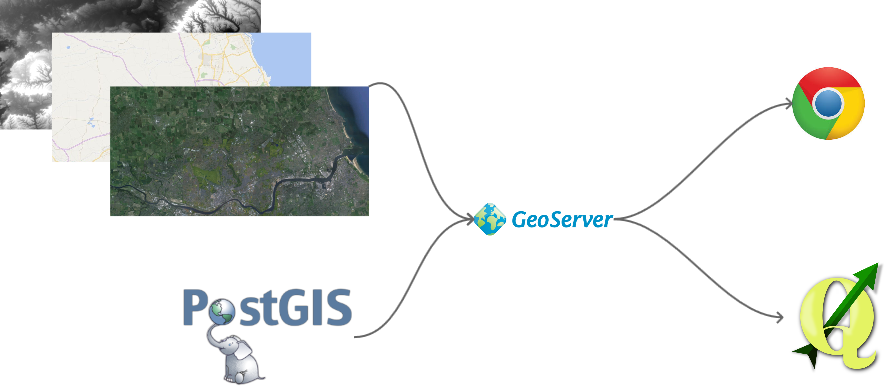
\includegraphics[width=1.0\textwidth]{webgis.png}}
\end{frame}

\begin{frame}{WebGIS}
	\begin{block}{A simple webmap to:}
		\begin{itemize}
			\item Publish select council datasets to the public and council staff
			\item Provide a means for staff to self-serve address data 
		\end{itemize}
	\end{block}	
\end{frame}


\begin{frame}{WebGIS}
	\begin{block}{A simple webmap to:}
		\begin{itemize}
			\item Publish select council datasets to the public and council staff
			\item Provide a means for staff to self-serve address data 
		\end{itemize}
	\end{block}	
\end{frame}

\section{Conclusions}
\begin{frame}{If you are considering Open Source GIS}
	\begin{block}{Considerations:}
		\begin{itemize}
			\item Planning
			\item Pilot study
			\item Data and service interoperability
			\item Cost...nothing is free
			\item Support
		\end{itemize}
	\end{block}	
\end{frame}

\begin{frame}{WebGIS}
	\begin{block}{Implementation:}
		\begin{itemize}
			\item All running on MS Windows
			\item PostGIS
			\item Geoserver + Geoserver Printing module
			\item Bespoke back-end services for
			\begin{itemize}
				\item Find my nearest
				\item Gazetteer
				\item Download
			\end{itemize}
			\item OpenLayers3
		\end{itemize}
	\end{block}	
\end{frame}




